\documentclass[journal,12pt,onecolumn]{IEEEtran}
\usepackage{cite}
\usepackage{graphicx}
\usepackage{amsmath,amssymb,amsfonts,amsthm}
\usepackage{algorithmic}
\usepackage{graphicx}
\usepackage{textcomp}
\usepackage{xcolor}
\usepackage{txfonts}
\usepackage{listings}
\usepackage{enumitem}
\usepackage{mathtools}
\usepackage{gensymb}
\usepackage{comment}
\usepackage[breaklinks=true]{hyperref}
\usepackage{tkz-euclide} 
\usepackage{listings}
\usepackage{gvv}                                        
%\def\inputGnumericTable{}                                 
\usepackage[latin1]{inputenc} 
\usetikzlibrary{arrows.meta, positioning}
\usepackage{xparse}
\usepackage{color}                                            
\usepackage{array}                                            
\usepackage{longtable}                                       
\usepackage{calc}                                             
\usepackage{multirow}
\usepackage{multicol}
\usepackage{hhline}                                           
\usepackage{ifthen}                                           
\usepackage{lscape}
\usepackage{tabularx}
\usepackage{array}
\usepackage{float}
\newtheorem{theorem}{Theorem}[section]
\newtheorem{problem}{Problem}
\newtheorem{proposition}{Proposition}[section]
\newtheorem{lemma}{Lemma}[section]
\newtheorem{corollary}[theorem]{Corollary}
\newtheorem{example}{Example}[section]
\newtheorem{definition}[problem]{Definition}
\newcommand{\BEQA}{\begin{eqnarray}}
\newcommand{\EEQA}{\end{eqnarray}}
\usepackage{float}
%\newcommand{\define}{\stackrel{\triangle}{=}}
\theoremstyle{remark}
\usepackage{circuitikz}
\usepackage{tikz}

\title{IN  INSTRUMENTATION ENGINEERING}
\author{EE25BTECH11031- Sai Sreevallabh}

\author{Sai Sreevallabh - ee25btech11031}

\begin{document}

\maketitle

\textbf{Q.$1$ to Q.$25$ Carry One Mark Each}

\begin{enumerate}

%1
\item The dimension of the null space of the matrix $\myvec{0 & 1 & 1 \\ 1 & 1 & 0 \\ 1 & 0 & 1}$ is
\par \hfill\brak{\text{GATE IN 2013}}
    \begin{enumerate}
    \begin{multicols}{4}
    \item $0$
    \item $1$
    \item $2$
    \item $3$
    \end{multicols}
    \end{enumerate}

%2
\item If the A-matrix of the state space model of a SISO linear time invariant system is rank deficient, the transfer function of the system must have
\par \hfill\brak{\text{GATE IN 2013}}
    \begin{enumerate}
    \begin{multicols}{2}
    \item a pole with a positive real part
    \item a pole with a negative real part
    \item a pole with a positive imaginary part
    \item a pole at the origin
    \end{multicols}
    \end{enumerate}

%3
\item Two systems with impulse responses $h_1\brak{t}$ and $h_2\brak{t}$ are connected in cascade. Then the overall impulse response of the cascaded system is given by
\par \hfill\brak{\text{GATE IN 2013}}
    \begin{enumerate}
    \begin{multicols}{2}
    \item product of $h_1\brak{t}$ and $h_2\brak{t}$
    \item sum of $h_1\brak{t}$ and $h_2\brak{t}$
    \item convolution of $h_1\brak{t}$ and $h_2\brak{t}$
    \item subtraction of $h_2\brak{t}$ from $h_1\brak{t}$
    \end{multicols}
    \end{enumerate}

%4
\item The complex function $\tanh \brak{s}$ is analytic over a region of the imaginary axis of the complex $s$-plane if the following is TRUE everywhere in the region for all integers $n$
\par \hfill\brak{\text{GATE IN 2013}}
    \begin{enumerate}
    \begin{multicols}{4}
    \item $\brak{\operatorname{Re}\brak{s}} = 0$
    \item $\brak{\operatorname{Im}\brak{s}} \ne n\pi$
    \item $\brak{\operatorname{Im}\brak{s}} \ne 3n\pi$
    \item $\brak{\operatorname{Im}\brak{s}} \ne (2n+1)\frac{\pi}{2}$
    \end{multicols}
    \end{enumerate}

%5
\item For a vector $E$, which one of the following statements is NOT TRUE?
\par \hfill\brak{\text{GATE IN 2013}}
    \begin{enumerate}
    \begin{multicols}{2}
    \item If $\nabla \cdot E = 0$, $E$ is called solenoidal.
    \item If $\nabla \times E = 0$, $E$ is called conservative.
    \item If $\nabla \times E = 0$, $E$ is called irrotational.
    \item If $\nabla \cdot E = 0$, $E$ is called irrotational.
    \end{multicols}
    \end{enumerate}

%6
\item For a periodic signal $v\brak{t} = 30 \sin 100 t + 10 \cos 300 t + 6 \sin\brak{500 t + \pi/4}$, the fundamental frequency in rad/s is
\par \hfill\brak{\text{GATE IN 2013}}
    \begin{enumerate}
    \begin{multicols}{4}
    \item $100$
    \item $300$
    \item $500$
    \item $1500$
    \end{multicols}
    \end{enumerate}

%7
\item In the transistor circuit as shown in \figref{7}, the value of resistance $R_E$ in k$\ohm$ is approximately,
\par \hfill\brak{\text{GATE IN 2013}}
\begin{figure}[H]
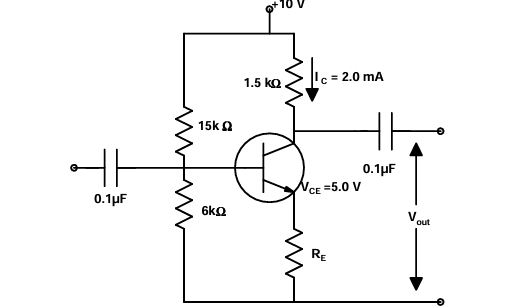
\includegraphics[width=0.5\columnwidth]{Figs/Q-7.png}
\caption{Transistor Circuit}
\label{7}
\end{figure}
    \begin{enumerate}
    \begin{multicols}{4}
    \item $1.0$
    \item $1.5$
    \item $2.0$
    \item $2.5$
    \end{multicols}
    \end{enumerate}

%8
\item A source $v_s\brak{t} = V \cos 100\pi t$ has an internal impedance of $4 + j 3\ \ohm$. If a purely resistive load connected to this source has to extract the maximum power, its value in $\ohm$ should be
\par \hfill\brak{\text{GATE IN 2013}}
    \begin{enumerate}
    \begin{multicols}{4}
    \item $3$
    \item $4$
    \item $5$
    \item $7$
    \end{multicols}
    \end{enumerate}

%9
\item Which one of the following statements is NOT TRUE for a continuous time causal and stable LTI system? 
\par \hfill\brak{\text{GATE IN 2013}}
    \begin{enumerate}
    \item All poles of the system must lie on the left side of the $j\omega$ axis.
    \item Zeros of the system can lie anywhere in the $s$-plane.
    \item All the poles must lie within $\abs{s}=1$.
    \item All roots of the characteristic equation must be located on the left side of the $j\omega$ axis.
    \end{enumerate}

%10
\item The operational amplifier shown in the circuit below in \figref{10} has a slew rate of $8.0\text{Volts}/\mu\text{s}$. The input signal is $0.25 \sin \brak{ \omega t}$. The maximum frequency of input in kHz for which there is no distortion in the output is
\par \hfill\brak{\text{GATE IN 2013}}
\begin{figure}[H]
\centering
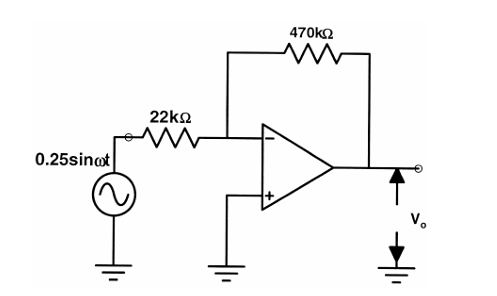
\includegraphics[width=0.5\columnwidth]{Figs/Q-10.png}
\caption{Operational Amplifier}
\label{10}
\end{figure}
    \begin{enumerate}
    \begin{multicols}{4}
    \item $23.84$
    \item $25.0$
    \item $50.0$
    \item $46.60$
    \end{multicols}
    \end{enumerate}

%11
\item Assuming zero initial condition, the response $y\brak{t}$ of the system given in \figref{11} to a unit step input $u\brak{t}$ is
\par \hfill\brak{\text{GATE IN 2013}}
\begin{figure}[H]
\centering
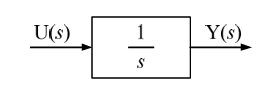
\includegraphics[width=0.2\columnwidth]{Figs/Q-11.png}
\caption{System}
\label{11}
\end{figure}
    \begin{enumerate}
    \begin{multicols}{4}
    \item $u\brak{t}$
    \item $t u\brak{t}$
    \item $\frac{t^2}{2} u\brak{t}$
    \item $e^{-t} u\brak{t}$
    \end{multicols}
    \end{enumerate}

\item The transfer function $\frac{V_2\brak{s}}{V_1\brak{s}}$ of the circuit shown below in \figref{12} is
\par \hfill\brak{\text{GATE IN 2013}}
\begin{figure}[H]
\centering
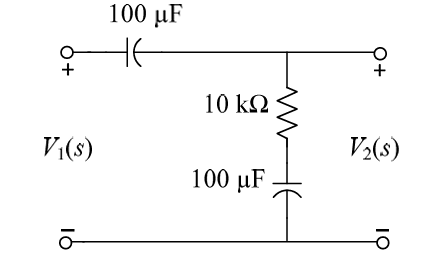
\includegraphics[width=0.3\columnwidth]{Figs/Q-12.png}
\caption{Circuit Diagram for Question 12}
\label{12}
\end{figure}
\begin{enumerate}
    \begin{multicols}{4}
    \item $\frac{0.5s+1}{s+1}$
    \item $\frac{3s+6}{s+2}$
    \item $\frac{s+2}{s+1}$
    \item $\frac{s+1}{s+2}$
    \end{multicols}
\end{enumerate}

\item The type of the partial differential equation $\frac{\partial f}{\partial t} = \frac{\partial^2 f}{\partial x^2}$ is
\par \hfill\brak{\text{GATE IN 2013}}
    \begin{enumerate}
    \begin{multicols}{4}
    \item Parabolic
    \item Elliptic
    \item Hyperbolic
    \item Nonlinear
    \end{multicols}
    \end{enumerate}

\item The discrete-time transfer function $\frac{1-2z^{-1}}{1-0.5z^{-1}}$ is
\par \hfill\brak{\text{GATE IN 2013}}
    \begin{enumerate}
    \item non-minimum phase and unstable.
    \item minimum phase and unstable.
    \item minimum phase and stable.
    \item non-minimum phase and stable.
    \end{enumerate}
%15
\item Match the following biomedical instrumentation techniques with their applications
\par \hfill\brak{\text{GATE IN 2013}}
\begin{multicols}{2}
    \begin{enumerate}[start = 16]
        \item Otoscopy
        \item Ultrasound Technique
        \item  Spirometry 
        \item Thermodilution Technique
    \end{enumerate}
        \columnbreak

        \begin{enumerate}[start = 21]
            \item Respiratory volume measurement
            \item Ear diagnostics 
            \item Echo-cardiography 
            \item Heart volume measurement 
        \end{enumerate}
\end{multicols}
    \begin{enumerate}
    \begin{multicols}{2}
    \item P-U, Q-V, R-X, S-W
    \item P-V, Q-U, R-X, S-W
    \item P-V, Q-W, R-U, S-X
    \item P-V, Q-W, R-X, S-U
    \end{multicols}
    \end{enumerate}

%16
\item A continuous random variable $X$ has a probability density function $f(x) = e^{-x}$, $0 < x < \infty$. Then $P\brak{X > 1}$ is  
\par \hfill\brak{\text{GATE IN 2013}}
\begin{enumerate}
\begin{multicols}{4}
\item $0.368$
\item $0.5$
\item $0.632$
\item $1.0$
\end{multicols}
\end{enumerate}

\item A band-limited signal with a maximum frequency of $5\,\text{kHz}$ is to be sampled. According to the sampling theorem, the sampling frequency in kHz which is not valid is  
\par \hfill\brak{\text{GATE IN 2013}}
\begin{enumerate}
\begin{multicols}{4}
\item $5$
\item $12$
\item $15$
\item $20$
\end{multicols}
\end{enumerate}

\item The differential pressure transmitter of a flow meter using a venturi tube reads $2.5 \times 10^5$ Pa for a flow rate of $0.5\,\text{m}^3/\text{s}$. The approximate flow rate in $\text{m}^3/\text{s}$ for a differential pressure $0.9 \times 10^5$ Pa is  
\par \hfill\brak{\text{GATE IN 2013}}
\begin{enumerate}
\begin{multicols}{4}
\item $0.30$
\item $0.18$
\item $0.83$
\item $0.60$
\end{multicols}
\end{enumerate}

%19
\item A bulb in a staircase has two switches, one switch being at the ground floor and the other one at the first floor. The bulb can be turned ON and also can be turned OFF by any one of the switches irrespective of the state of the other switch. The logic of switching of the bulb resembles  
\par \hfill\brak{\text{GATE IN 2013}}
\begin{enumerate}
\begin{multicols}{4}
\item an AND gate
\item an OR gate
\item an XOR gate
\item a NAND gate
\end{multicols}
\end{enumerate}

\item The impulse response of a system is $h\brak{t} = t u\brak{t}$. For an input $u\brak{t-1}$, the output is  
\par \hfill\brak{\text{GATE IN 2013}}
\begin{enumerate}
\begin{multicols}{4}
\item $\frac{t^{2}}{2} u\brak{t}$
\item $t\brak{t-1} u\brak{t-1}$
\item $\brak{t-1}^{2} u\brak{t}$
\item $\frac{\brak{t^2-1}}{2} u\brak{t-1}$
\end{multicols}
\end{enumerate}

%21
\item Consider a delta connection of resistors and its equivalent star connection as shown in \figref{21}. If all elements of the delta connection are scaled by a factor $k$, $k > 0$, the elements of the corresponding star equivalent will be scaled by a factor of 
\par \hfill\brak{\text{GATE IN 2013}}
\begin{figure}[H]
    \centering
    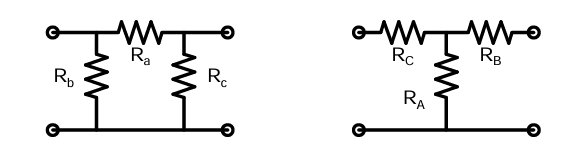
\includegraphics[width=0.5\columnwidth]{Figs/Q-21.png}
    \caption{Star and Delta Connections}
    \label{21}
\end{figure}
\begin{enumerate}
\begin{multicols}{4}
\item $k^{2}$
\item $k$
\item $\frac{1}{k}$
\item $\sqrt{k}$
\end{multicols}
\end{enumerate}

%22
\item An accelerometer has input range of $0$ to $10g$, natural frequency $30 \,\text{Hz}$ and mass $0.001\,\text{kg}$. The range of the secondary displacement transducer in mm required to cover the input range is  
\par \hfill\brak{\text{GATE IN 2013}}
\begin{enumerate}
\begin{multicols}{4}
\item $0$ to $2.76$
\item $0$ to $9.81$
\item $0$ to $11.20$
\item $0$ to $52.10$
\end{multicols}
\end{enumerate}

\item In the circuit shown below what is the output voltage $V_{\text{out}}$ in Volts if a silicon transistor Q and an ideal op-amp are used?  
\par \hfill\brak{\text{GATE IN 2013}}
\begin{figure}[H]
\centering
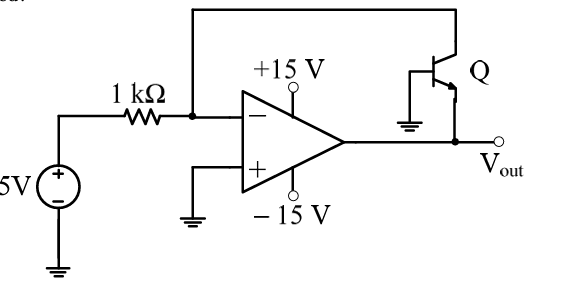
\includegraphics[width=0.5\columnwidth]{Figs/Q-23.png}
\caption{Circuit Diagram for Question-23}
\label{23}
\end{figure}
\begin{enumerate}
\begin{multicols}{4}
\item $-15$
\item $-0.7$
\item $+0.7$
\item $+15$
\end{multicols}
\end{enumerate}

\item In the feedback network shown in \figref{24}, if the feedback factor $k$ is increased, then the  
\par \hfill\brak{\text{GATE IN 2013}}
\begin{figure}[H]
    \centering
    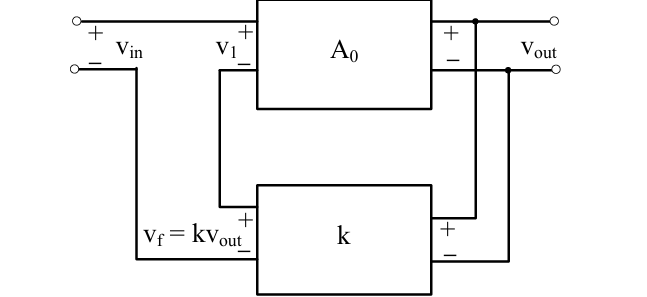
\includegraphics[width=0.5\linewidth]{Figs/Q-24.png}
    \caption{Feedback Network}
    \label{24}
\end{figure}
\begin{enumerate}
\item input impedance increases and output impedance decreases
\item input impedance increases and output impedance also increases
\item input impedance decreases and output impedance also decreases
\item input impedance decreases and output impedance increases
\end{enumerate}

%25
\item The Bode plot of a transfer function $G\brak{s}$ is shown in \figref{25}. The gain $\brak{20 \log \abs{G\brak{s}}}$ is $32\,\text{dB}$ and $-8\,\text{dB}$ at $1\,\text{rad/s}$ and $10\,\text{rad/s}$ respectively. The phase is negative for all $\omega$. Then $G\brak{s}$ is  
\par \hfill\brak{\text{GATE IN 2013}}
\begin{figure}[H]
    \centering
    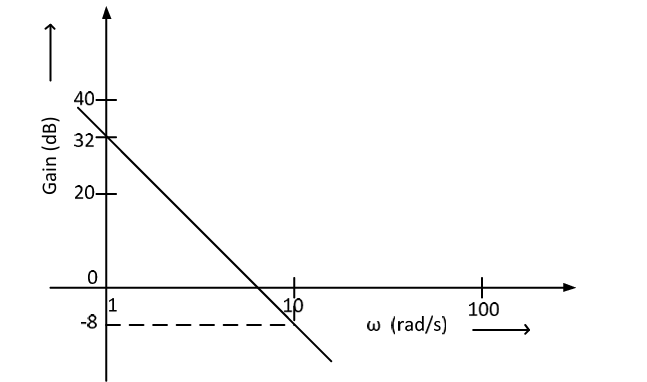
\includegraphics[width=0.5\linewidth]{Figs/Q-25.png}
    \caption{Bode Plot}
    \label{25}
\end{figure}
\begin{enumerate}
\begin{multicols}{4}
\item $\frac{39.8}{s}$
\item $\frac{39.8}{s^2}$
\item $\frac{32}{s}$
\item $\frac{32}{s^2}$
\end{multicols}
\end{enumerate}

\textbf{Q.$26$ to Q.$55$ Carry Two Marks Each}

%26
\item While numerically solving the differential equation $\frac{dy}{dx} + 2xy^2 = 0, \quad y(0) = 1$
using Euler's predictor-corrector (improved Euler-Cauchy) method with a step size of $0.2$, the value of $y$ after the first step is  
\par \hfill\brak{\text{GATE IN 2013}}
\begin{enumerate}
\begin{multicols}{4}
\item $1.00$
\item $1.03$
\item $0.97$
\item $0.96$
\end{multicols}
\end{enumerate}

%27
\item One pair of eigenvectors corresponding to the two eigenvalues of the matrix $\myvec{0 & 1 \\ 1 & 0}$ is  
\par \hfill\brak{\text{GATE IN 2013}}
\begin{enumerate}
\begin{multicols}{4}
\item $\myvec{-1 \\ -j}, \myvec{1 \\ j}$
\item $\myvec{0 \\ 1}, \myvec{-1 \\ 0}$
\item $\myvec{1 \\ j}, \myvec{0 \\ 1}$
\item $\myvec{1 \\ j}, \myvec{j \\ 1}$
\end{multicols}
\end{enumerate}

%28
\item The digital circuit shown in \figref{28} uses two negative edge-triggered D-flip-flops. Assuming initial condition of $Q_1$ and $Q_0$ as zero, the output $Q_1 Q_0$ of this circuit is  
\par \hfill\brak{\text{GATE IN 2013}}
\begin{figure}[H]
\centering
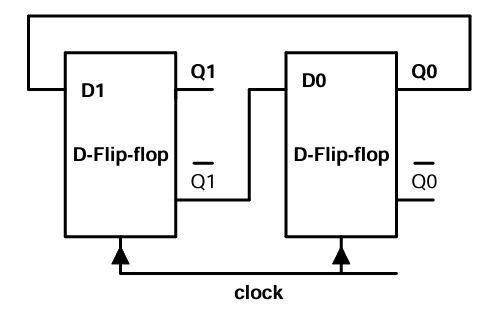
\includegraphics[width=0.5\columnwidth]{Figs/Q-28.png}
\caption{Digital Circuit}
\label{28}
\end{figure}
\begin{enumerate}
\begin{multicols}{4}
\item $00, 01, 10, 11, 00 \dots$
\item $00, 01, 11, 10, 00 \dots$
\item $00, 11, 10, 01, 00 \dots$
\item $00, 01, 11, 11, 00 \dots$
\end{multicols}
\end{enumerate}

\item Considering the transformer to be ideal, the transmission parameter 'A' of the 2-port network shown in \figref{29} is  
\par \hfill\brak{\text{GATE IN 2013}}
\begin{figure}[H]
\centering
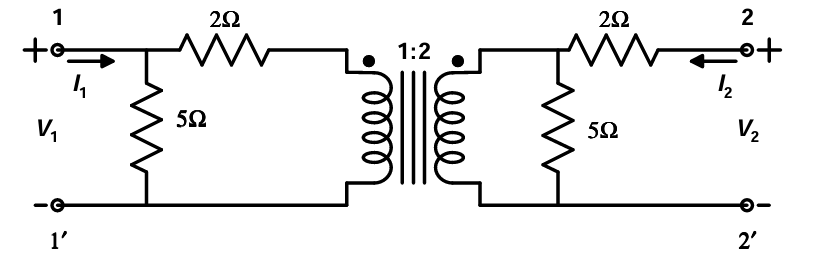
\includegraphics[width=0.5\columnwidth]{Figs/Q-29.png}
\caption{Transformer}
\label{29}
\end{figure}
\begin{enumerate}
\begin{multicols}{4}
\item $1.3$
\item $1.4$
\item $0.5$
\item $2.0$
\end{multicols}
\end{enumerate}

%30
\item The following arrangement consists of an ideal transformer and an attenuator, as shown in \figref{30}, which attenuates by a factor of $0.8$. An AC voltage $V_{WX 1} = 100\,\text{V}$ is applied across WX to get an open circuit voltage $V_{YZ1}$ across YZ. Next, an AC voltage $V_{YZ2} = 100\,\text{V}$ is applied across YZ to get an open circuit voltage $V_{WX 2}$ across WX. Then $\frac{V_{YZ1}}{V_{WX1}}$ and $\frac{V_{WX2}}{V_{YZ2}}$ are respectively,  
\par \hfill\brak{\text{GATE IN 2013}}
\begin{figure}[H]
\centering
    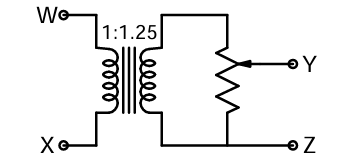
\includegraphics[width=0.5\linewidth]{Figs/Q-30.png}
    \caption{Ideal Transformer}
    \label{30}
\end{figure}
\begin{enumerate}
\begin{multicols}{4}
\item $\frac{125}{100}$ and $\frac{80}{100}$
\item $\frac{100}{100}$ and $\frac{80}{100}$
\item $\frac{100}{100}$ and $\frac{100}{100}$
\item $\frac{80}{100}$ and $\frac{80}{100}$
\end{multicols}
\end{enumerate}

%31
\item The open-loop transfer function of a DC motor is given as  
$\frac{V_{\omega}\brak{s}}{V_a\brak{s}} = \frac{10}{1 + 10s}$

When connected in feedback as shown in \figref{31} the approximate value of $K_a$ that will reduce the time constant of the closed loop system by one hundred times as compared to that of the open-loop system is  
\par \hfill\brak{\text{GATE IN 2013}}
\begin{figure}[H]
\centering
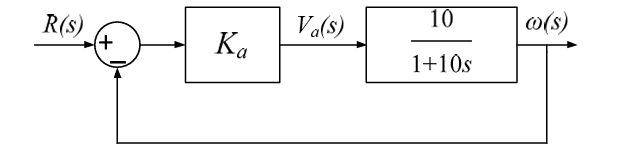
\includegraphics[width=0.5\columnwidth]{Figs/Q-31.png}
\caption{Diagram for Question-31}
\label{31}
\end{figure}
\begin{enumerate}
\begin{multicols}{4}
\item $1$
\item $5$
\item $10$
\item $100$
\end{multicols}
\end{enumerate}

%32
\item  Two magnetically uncoupled inductive coils have $Q$ factors $q_1$ and $q_2$ at the chosen operating frequency. Their respective resistances are $R_1$ and $R_2$. When connected in series, the effective $Q$ factor of the series combination at the same operating frequency is \par \hfill\brak{\text{GATE IN 2013}}
\begin{enumerate}
\begin{multicols}{2}
    \item $q_1 + q_2$
    \item $\brak{1/q_1}+\brak{1/q_2}$
    \item $\brak{q_1R_1+q_2R_2}/\brak{R_1+R_2}$
    \item $\brak{q_1R_2+q_2R_1}/\brak{R_1+R_2}$
\end{multicols}
\end{enumerate}

%33
\item For the circuit shown in \figref{33}, the knee current of the ideal Zener diode is $10\,\text{mA}$. To maintain $5\,\text{V}$ across $R_L$, the minimum value of the load resistor $R_L$ in $\ohm$ and the minimum power rating of the Zener diode in mW, respectively, are  
\par \hfill\brak{\text{GATE IN 2013}}
\begin{figure}[H]
\centering
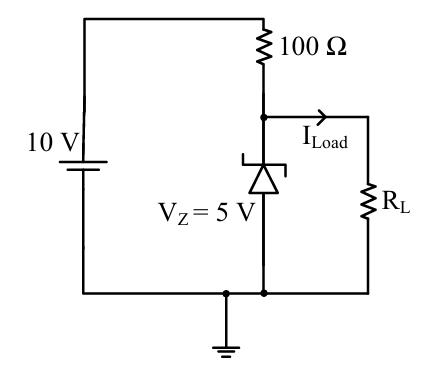
\includegraphics[width=0.3\columnwidth]{Figs/Q-33.png}
\caption{Circuit Diagram for Question-33}
\label{33}
\end{figure}
\begin{enumerate}
\begin{multicols}{4}
\item $125$ and $125$
\item $125$ and $250$
\item $250$ and $125$
\item $250$ and $250$
\end{multicols}
\end{enumerate}

%34
\item The impulse response of a continuous time system is given by $h\brak{t} = \delta\brak{t-1} + \delta\brak{t-3}$. The value of the step response at $t = 2$ is  
\par \hfill\brak{\text{GATE IN 2013}}
\begin{enumerate}
\begin{multicols}{4}
\item $0$
\item $1$
\item $2$
\item $3$
\end{multicols}
\end{enumerate}

\item Signals from fifteen thermocouples are multiplexed and each one is sampled once per second with a 16-bit ADC. The digital samples are converted by a parallel to serial converter to generate a serial PCM signal. This PCM signal is frequency modulated with FSK modulator with $1200\,\text{Hz}$ as $1$ and $960\,\text{Hz}$ as $0$. The minimum band allocation required for faithful reproduction of the signal by the FSK receiver without considering noise is  
\par \hfill\brak{\text{GATE IN 2013}}
\begin{enumerate}
\begin{multicols}{4}
\item $840\, \text{Hz}$ to $1320\, \text{Hz}$
\item $960\, \text{Hz}$ to $1200\, \text{Hz}$
\item $1080\, \text{Hz}$ to $1320\, \text{Hz}$
\item $720\, \text{Hz}$ to $1440\, \text{Hz}$
\end{multicols}
\end{enumerate}

\item Three capacitors $C_1, C_2$ and $C_3$ whose values are $10\,\mu\text{F}$, $5\,\mu\text{F}$, and $2\,\mu\text{F}$ respectively, have breakdown voltages of $10\,\text{V}$, $5\,\text{V}$, and $2\,\text{V}$ respectively. For the interconnection shown in \figref{36}, the maximum safe voltage in Volts that can be applied across the combination, and the corresponding total charge in $\mu C$ stored in the effective capacitance across the terminals are, respectively,  
\par \hfill\brak{\text{GATE IN 2013}}
\begin{figure}[H]
\centering
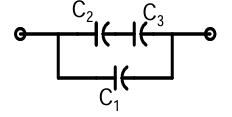
\includegraphics[width=0.3\columnwidth]{Figs/Q-36.png}
\caption{Combination fo Capcitors}
\label{36}
\end{figure}
\begin{enumerate}
\begin{multicols}{4}
\item $2.8$ and $36$
\item $7$ and $119$
\item $2.8$ and $32$
\item $7$ and $80$
\end{multicols}
\end{enumerate}

\item The maximum value of the solution $y\brak{t}$ of the differential equation $y''\brak{t} + y\brak{t} = 0$ with initial conditions $y'\brak{0} =1$ and $y\brak{0} = 1$ for $t \ge 0$ is  
\par \hfill\brak{\text{GATE IN 2013}}
\begin{enumerate}
\begin{multicols}{4}
\item $1$
\item $2$
\item $\pi$
\item $\sqrt{2}$
\end{multicols}
\end{enumerate}

%38
\item The Laplace Transform representation of the triangular pulse shown in \figref{38} is \par \hfill\brak{\text{GATE IN 2013}}
\begin{figure}[H]
    \centering
    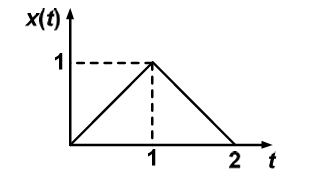
\includegraphics[width=0.4\linewidth]{Figs/Q-38.png}
    \caption{Triangular Pulse}
    \label{38}
\end{figure}
\begin{enumerate}
\begin{multicols}{2}
\item $\frac{1}{s^2}\sbrak{1+e^{-2s}}$
\item $\frac{1}{s^2}\sbrak{1-e^{-s}+e^{-2s}}$
\item $\frac{1}{s^2}\sbrak{1-e^{-s}+2e^{-2s}}$
\item $\frac{1}{s^2}\sbrak{1-2e^{-s}+e^{-2s}}$
\end{multicols}
\end{enumerate}

%39
\item In the circuit shown in \figref{39}, if the source voltage $V_S = 100 \angle 53.13^{\degree}$ Volts, then the Thevenin's equivalent voltage in Volts as seen by the load resistance $R_L$ is  
\par \hfill\brak{\text{GATE IN 2013}}
\begin{figure}[H]
\centering
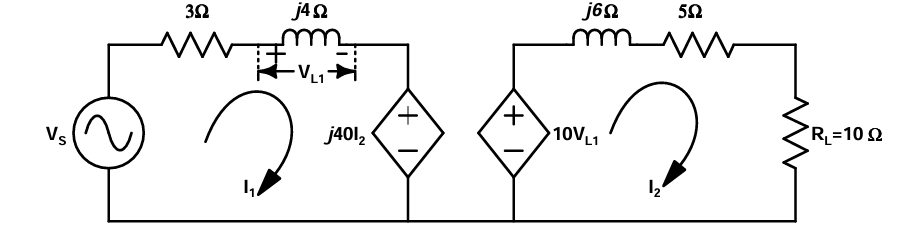
\includegraphics[width=0.7\columnwidth]{Figs/Q-39.png}
\caption{Circuit Diagram for Question-39}
\label{39}
\end{figure}
\begin{enumerate}
\begin{multicols}{4}
\item $100 \angle 90{\degree}$
\item $800 \angle 0{\degree}$
\item $800 \angle 90{\degree}$
\item $100 \angle 60{\degree}$
\end{multicols}
\end{enumerate}

%40
\item A signal $v_i\brak{t} = 10+ \sin 100 \pi t + \sin 4000 \pi t + \sin 100000 \pi t$ is supplied to a filter circuit (shown below) made up of ideal op-amps. The least attenuated frequency component in the output will be  
\par \hfill\brak{\text{GATE IN 2013}}
\begin{figure}[H]
\centering
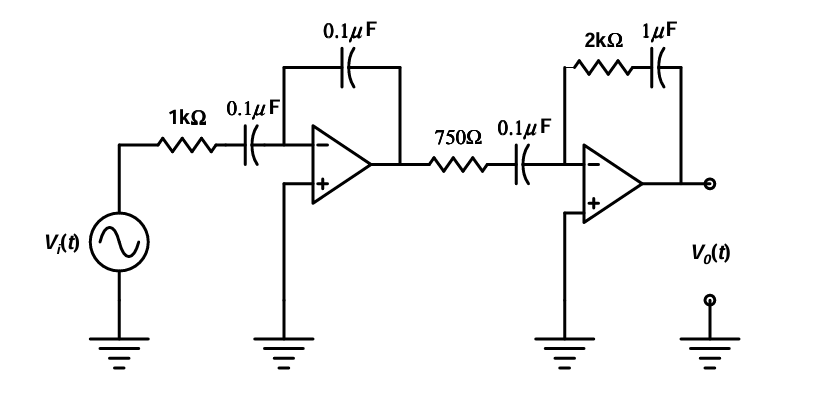
\includegraphics[width=0.6\columnwidth]{Figs/Q-40.png}
\caption{Circuit Diagram for Question-40}
\label{40}
\end{figure}
\begin{enumerate}
\begin{multicols}{4}
\item $0\,\text{Hz}$
\item $50\,\text{Hz}$
\item $2\,\text{kHz}$
\item $50\,\text{kHz}$
\end{multicols}
\end{enumerate}

%41
\item The signal flow graph for a system is given in \figref{41}. The transfer function $\frac{Y\brak{s}}{U\brak{s}}$ for this system is given as  
\par \hfill\brak{\text{GATE IN 2013}}
\begin{figure}[H]
\centering
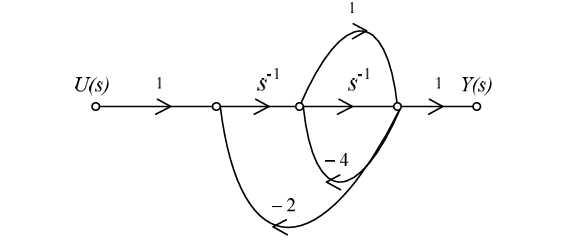
\includegraphics[width=0.5\columnwidth]{Figs/Q-41.png}
\caption{Signal Flow Graph}
\label{41}
\end{figure}
\begin{enumerate}
    \begin{multicols}{2}
    \item $\frac{s+1}{5s^{2}+6s+2}$
    \item $\frac{s+1}{s^{2}+6s+2}$
    \item $\frac{s+1}{s^{2}+4s+2}$
    \item $\frac{1}{5s^{2}+6s+2}$
    \end{multicols}
\end{enumerate}

%42
\item A voltage $1000 \sin \omega t$ Volts is applied across YZ shown in \figref{42}. Assuming ideal diodes, the voltage measured across WX in Volts, is 
\begin{figure}[H]
    \centering
    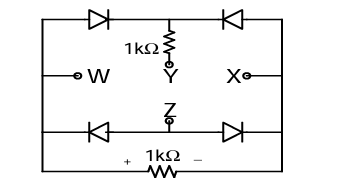
\includegraphics[width=0.4\linewidth]{Figs/Q-42.png}
    \caption{Circuit Diagram for Question-42}
    \label{42}
\end{figure}
\par \hfill\brak{\text{GATE IN 2013}}
\begin{enumerate}
    \begin{multicols}{2}
    \item $\sin \omega t$
    \item $\brak{\sin \omega t + \abs{\sin \omega t}}/2$
    \item $\brak{\sin \omega t - \abs{\sin \omega t}}/2$
    \item $0$ for all $t$
    \end{multicols}
\end{enumerate}

%43
\item In the circuit shown in \figref{43} the op-amps are ideal. Then $V_{\text{out}}$ in Volts is  
\par \hfill\brak{\text{GATE IN 2013}}
\begin{figure}[H]
\centering
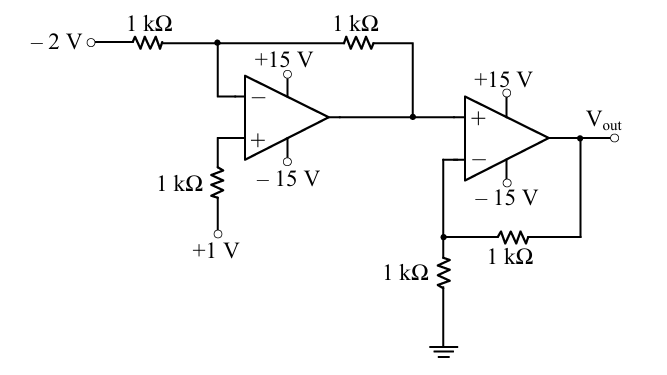
\includegraphics[width=0.6\columnwidth]{Figs/Q-43.png}
\caption{Circuit Diagram for Question-43}
\label{43}
\end{figure}
\begin{enumerate}
\begin{multicols}{4}
\item $4$
\item $6$
\item $8$
\item $10$
\end{multicols}
\end{enumerate}

%44
\item In the circuit shown in \figref{44}, $Q_1$ has negligible collector-to-emitter saturation voltage and the diode drops negligible voltage across it under forward bias. If $V_{cc}$ is $+5\,\text{V}$, $X$ and $Y$ are digital signals with $0$ V as logic $0$ and $V_{cc}$ as logic $1$, then the Boolean expression for $Z$ is  \par \hfill\brak{\text{GATE IN 2013}}
\begin{figure}[H]
    \centering
    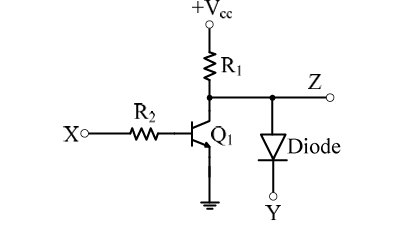
\includegraphics[width=0.5\linewidth]{Figs/Q-44.png}
    \caption{Circuit Diagram for Question-44}
    \label{44}
\end{figure}
\begin{enumerate}
\begin{multicols}{4}
\item $X Y$
\item $\overline{X}Y$
\item $X \overline{Y}$
\item $\overline{XY}$
\end{multicols}
\end{enumerate}

%45
\item The circuit below incorporates a permanent magnet moving coil milli-ammeter of range $1\,\text{mA}$ having a series resistance of $10\,k\ohm$. Assuming constant diode forward resistance of $50\,\ohm$, a forward diode drop of $0.7\,\text{V}$ and infinite reverse diode resistance for each diode, the reading of the meter in mA is  
\par \hfill\brak{\text{GATE IN 2013}}
\begin{figure}[H]
\centering
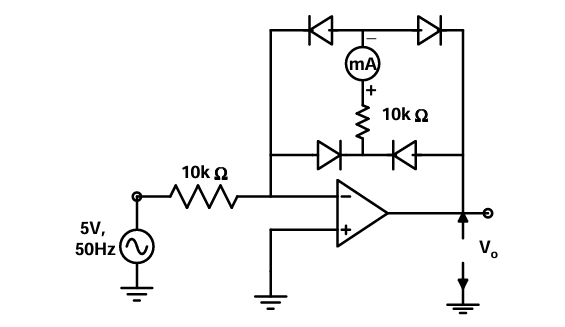
\includegraphics[width=0.5\columnwidth]{Figs/Q-45.png}
\caption{Circuit Diagram for Question-45}
\label{45}
\end{figure}
\begin{enumerate}
\begin{multicols}{4}
\item $0.45$
\item $0.5$
\item $0.7$
\item $0.9$
\end{multicols}
\end{enumerate}

%46
\item Measurement of optical absorption of a solution is disturbed by the additional stray light falling at the photo-detector. For estimation of the error caused by stray light the following data could be obtained from controlled experiments.  
\quad Photo-detector output without solution and without stray light is $500\,\mu W$.  
\quad Photo-detector output without solution and with stray light is $600\,\mu W$.  
\quad Photo-detector output with solution and with stray light is $200\,\mu W$.  
The percent error in computing absorption coefficient due to stray light is  
\par \hfill\brak{\text{GATE IN 2013}}
\begin{enumerate}
\begin{multicols}{4}
\item $12.50$
\item $31.66$
\item $33.33$
\item $94.98$
\end{multicols}
\end{enumerate}

%47
\item Two ammeters $A_1$ and $A_2$ measure the same current and provide readings $I_1$ and $I_2$, respectively. The ammeter errors can be characterized as independent zero mean Gaussian random variables of standard deviations $\sigma_1$ and $\sigma_2$, respectively. The value of the current is computed as :  
$$
I = \mu I_1 + (1 - \mu) I_2
$$
The value of $\mu$ which gives the lowest standard deviation of $I$ is  
\par \hfill\brak{\text{GATE IN 2013}}
\begin{enumerate}
\begin{multicols}{4}
\item $\frac{\sigma_2^{2}}{\sigma_1^{2} + \sigma_2^{2}}$
\item $\frac{\sigma_1^{2}}{\sigma_1^{2} + \sigma_2^{2}}$
\item $\frac{\sigma_1}{\sigma_1 + \sigma_2}$
\item $\frac{\sigma_1}{\sigma_1 + \sigma_2}$
\end{multicols}
\end{enumerate}

\section*{Common Data Questions}

\textbf{Common Data for 48 and 49}

A tungsten wire used in a constant current hot wire anemometer has the following parameters : \\
Resistance at $0 \degree C$ is $10 \ohm$, Surface area is $10^{-4} m^2$, Linear temperature coefficient of resistance of the tungsten wire is $3 \times 4.8 \times 10^{-3} / \degree C$, Convective heat transfer coefficient is $25.2 W/m^2 / \degree C$, flowing air temperature is $30 \degree C$, wire current is $100\,mA$, mass-specific heat product is $2.5 \times 10^{-5} J / \degree C$.

\item The thermal time constant of the hot wire under flowing air condition in ms is  
\par \hfill\brak{\text{GATE IN 2013}}
\begin{enumerate}
\begin{multicols}{4}
\item $24.5$
\item $12.25$
\item $6.125$
\item $3.0625$
\end{multicols}
\end{enumerate}

\item At steady state, the resistance of the wire in $\ohm$ is  
\par \hfill\brak{\text{GATE IN 2013}}
\begin{enumerate}
\begin{multicols}{4}
\item $10.000$
\item $10.144$
\item $12.152$
\item $14.128$
\end{multicols}
\end{enumerate}

\textbf{Common Data for Questions 50 and 51}

A piezo-electric force sensor, connected by a cable to a voltage amplifier, has the following parameters :\\
Crystal stiffness $10^9\,\text{N/m}$, Damping ratio $0.01$, Natural frequency $10^5\,\text{rad/s}$, Force-to-Charge sensitivity $9 \times 10^{-9} \text{C/N}$, Capacitance $9 \times 10^{-9} \text{F}$ with its loss angle assumed negligible. \\
Cable capacitance $2 \times 10^{-9} \text{F}$ with its resistance assumed negligible.\\
Amplifier properties: Input impedance $1\,\text{M}\ohm$, Bandwidth $1\,\text{MHz}$, Gain $3$.

\item The maximum frequency of a force signal in Hz below the natural frequency within its useful mid-band range of measurement, for which the gain amplitude is less than $1.05$, approximately is,  
\par \hfill\brak{\text{GATE IN 2013}}
\begin{enumerate}
\begin{multicols}{4}
\item $35$
\item $350$
\item $3500$
\item $16 \times 10^{3}$
\end{multicols}
\end{enumerate}

%51
\item The minimum frequency of a force signal in Hz within its useful mid-band range of measurement, for which the gain amplitude is more than $0.95$, approximately is,  
\par \hfill\brak{\text{GATE IN 2013}}
\begin{enumerate}
\begin{multicols}{4}
\item $16$
\item $160$
\item $1600$
\item $16 \times 10^{3}$
\end{multicols}
\end{enumerate}

\section*{Linked Answer Questions}

\textbf{Statement for Linked Answer Questions 52 and 53}
Consider a plant with the transfer function  
$G\brak{s} = \frac{1}{s+1}^3$ 
Let $K_u$ and $T_u$ be the ultimate gain and ultimate period corresponding to the frequency response-based closed loop Ziegler-Nichols cycling method, respectively. The Ziegler-Nichols tuning rule for a P-controller is given as:  
$K_p = 0.5 K_u.$

\item The values of $K_u$ and $T_u$, respectively, are  
\par \hfill\brak{\text{GATE IN 2013}}
\begin{enumerate}
\begin{multicols}{4}
\item $2\sqrt{2}, 2 \pi$
\item $8, 2 \pi$
\item $8, \frac{2 \pi}{3}$
\item $2\sqrt{2}, \frac{2 \pi}{3}$
\end{multicols}
\end{enumerate}

\item The gain of the transfer function between the plant output and an additive load disturbance input of frequency $\frac{2 \pi}{T_u}$ in closed loop with a P-controller designed according to the Ziegler-Nichols tuning rule as given above is  
\par \hfill\brak{\text{GATE IN 2013}}
\begin{enumerate}
\begin{multicols}{4}
\item $-1.0$
\item $0.5$
\item $1.0$
\item $2.0$
\end{multicols}
\end{enumerate}

\textbf{Statement for Linked Answer Questions 54 and 55}

 A differential amplifier with signal terminals $X, Y, Z$ is connected as shown in \figref{54} below for CMRR measurement where the differential amplifier has an additional constant offset voltage in the output. The observations obtained are: when $V_0 = 2\,mV$, $V_i = 3\,mV$, and when $V_0 = 3\,mV$, $V_i = 4\,mV$.  
\begin{figure}[H]
\centering
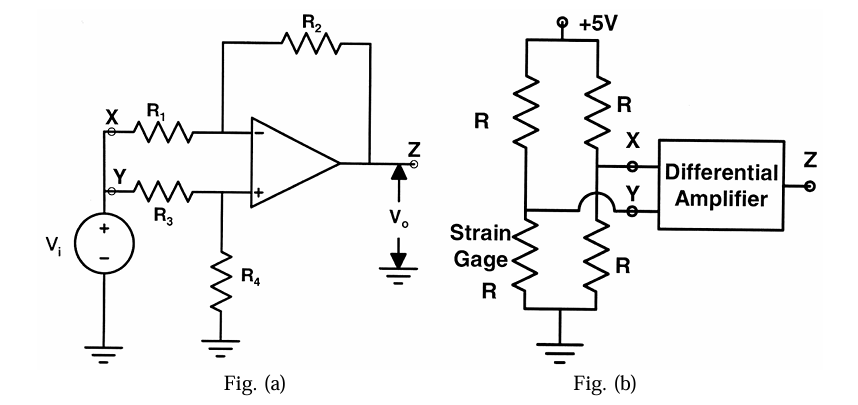
\includegraphics[width=0.6\columnwidth]{Figs/Q-54&55.png}
\caption{Circuit Diagram}
\label{54}
\end{figure}

\item Assuming its differential gain to be $10$ and the op-amp to be otherwise ideal, the CMRR is  
\par \hfill\brak{\text{GATE IN 2013}}
\begin{enumerate}
\begin{multicols}{4}
\item $10^2$
\item $10^3$
\item $10^4$
\item $10^5$
\end{multicols}
\end{enumerate}

\item The differential amplifier is connected as shown in Fig. (b) above to a single strain gage bridge. Let the strain gage resistance vary around its no-load resistance $R$ by $\pm 1\%$. Assume the input impedance of the amplifier to be high compared to the equivalent source resistance of the bridge, and the common mode characteristic to be as obtained above. The output voltage in mV varies approximately from  
\par \hfill\brak{\text{GATE IN 2013}}
\begin{enumerate}
\begin{multicols}{4}
\item $+128$ to $-128$
\item $+128$ to $-122$
\item $+122$ to $-122$
\item $+99$ to $-101$
\end{multicols}
\end{enumerate}

\section*{GENERAL APTITUDE}

\textbf{Q.56 to Q.60 carry one mark each}

\item Statement: You can always give me a ring whenever you need. Which one of the following is the best inference from the above statement?  
\par \hfill\brak{\text{GATE IN 2013}}
\begin{enumerate}
\item Because I have a nice caller tune.
\item Because I have a better telephone facility.
\item Because a friend in need is a friend indeed.
\item Because you need not pay towards the telephone bills when you give me a ring.
\end{enumerate}

\item Complete the sentence: Dare \rule{1.5cm}{0.4pt} mistakes.  
\par \hfill\brak{\text{GATE IN 2013}}
\begin{enumerate}
\begin{multicols}{4}
\item commit
\item to commit
\item committed
\item committing
\end{multicols}
\end{enumerate}

\item Choose the grammatically CORRECT sentence:  
\par \hfill\brak{\text{GATE IN 2013}}
\begin{enumerate}
\begin{multicols}{2}
\item Two and two add four.
\item Two and two become four.
\item Two and two are four.
\item Two and two make four.
\end{multicols}
\end{enumerate}

\item They were requested not to \textbf{quarrel} with others. Which one of the following options is the closest in meaning to the word \textbf{quarrel}?  
\par \hfill\brak{\text{GATE IN 2013}}
\begin{enumerate}
\begin{multicols}{4}
\item make out
\item call out
\item dig out
\item fall out
\end{multicols}
\end{enumerate}

\item In the summer of 2012, in New Delhi, the mean temperature of Monday to Wednesday was $41 \degree$ C and of Tuesday to Thursday was $43 \degree$ C. If the temperature on Thursday was 15\% higher than that of Monday, then the temperature in $\degree C$ on Thursday was  
\par \hfill\brak{\text{GATE IN 2013}}
\begin{enumerate}
\begin{multicols}{4}
\item $40$
\item $43$
\item $46$
\item $49$
\end{multicols}
\end{enumerate}

\textbf{Q.61 to Q.65 carry two marks each}

\item Find the sum to $n$ terms of the series $10 + 84 + 734 + \ldots$
\par \hfill\brak{\text{GATE IN 2013}}
\begin{enumerate}
    \begin{multicols}{2}
    \item $\frac{9\brak{9^{n} + 1}}{10} + 1$
    \item $\frac{9\brak{9^{n} - 1}}{8} + 1$
    \item $\frac{9\brak{9^{n} - 1}}{8} + n$
    \item $\frac{9\brak{9^{n} - 1}}{8} + n^{2}$
    \end{multicols}
\end{enumerate}


\item The set of values of $p$ for which the roots of the equation $3x^2 + 2x + p\brak{p - 1} = 0$ are of opposite sign is  
\par \hfill\brak{\text{GATE IN 2013}}
\begin{enumerate}
\begin{multicols}{4}
\item $(-\infty, 0)$
\item $(0, 1)$
\item $(1, \infty)$
\item $(0, \infty)$
\end{multicols}
\end{enumerate}

\item A car travels $8\,\text{km}$ in the first quarter of an hour, $6\,\text{km}$ in the second quarter and $16\,\text{km}$ in the third quarter. The average speed of the car in km per hour over the entire journey is  
\par \hfill\brak{\text{GATE IN 2013}}
\begin{enumerate}
\begin{multicols}{4}
\item $30$
\item $36$
\item $40$
\item $24$
\end{multicols}
\end{enumerate}

\item What is the chance that a leap year, selected at random, will contain 53 Saturdays?  
\par \hfill\brak{\text{GATE IN 2013}}
\begin{enumerate}
\begin{multicols}{4}
\item $\frac{2}{7}$
\item $\frac{3}{7}$
\item $\frac{1}{7}$
\item $\frac{5}{7}$
\end{multicols}
\end{enumerate}

\item Statement: There were different streams of freedom movements in colonial India carried out by the moderates, liberals, radicals, socialists, and so on. Which one of the following is the best inference from the above statement?  
\par \hfill\brak{\text{GATE IN 2013}}
\begin{enumerate}
\item The emergence of nationalism in colonial India led to our Independence.
\item Nationalism in India emerged in the context of colonialism.
\item Nationalism in India is homogeneous.
\item Nationalism in India is heterogeneous.
\end{enumerate}

\end{enumerate}

\end{document}
